%%
%% This is file `article1.tex', % generated with the docstrip utility.
%%
%% The original source files were:
%%
%% dms.dtx  (with options: `article') % Example TeX file for the documentation %
%of the jurabib package % Copyright (C) 1999, 2000, 2001 Jens Berger % See
%dms.ins  for the copyright details.
%% 
%%% ====================================================================
%%%  @LaTeX-file{ %%     filename        = "dms.dtx", %%     author    =
%"Nicolas Beauchemin, Damien Rioux-Lavoie, Victor Fardel, Jonathan Godin", %%
%copyright = "Copyright (C) 2000 , DMS %%                  all rights reserved.
%Copying of this file is %%                  authorized only if either: %%
%(1) you make absolutely no changes to your copy, %%                  including
%name; OR %%                  (2) if you do make changes, you first rename it %%
%to some other name.", %%     address   = "Département de Mathématiques et de
%Statistique", %%     telephone = "514-343-6705", %%     FAX       =
%"514-343-5700", %%     email     = "aide@dms.umontreal.ca (Internet)", %%
%keywords  = "latex, amslatex, ams-latex, theorem", %%     abstract  = " Ce
%fichier est un package conçu pour être %%                  utilisé avec la
%version de LaTeX2e 1995/06/01. Il %%                  est prévue pour la classe
%``amsbook''. Il en %%                  modifie le format des pages, l'entête
%des %%                  sections, etc, afin d'être  conforme au modèle de %%
%mémoire de maîtrise de l'Université de %%                  Montréal. Finalement
%ce fichier est grandement %%                  inspiré du fichier
%amsclass.dtx.", %%     docstring = "The checksum field contains: CRC-16
%checksum, %%                  word count, line count, and character count, as
%%%                  produced by Robert Solovay's checksum utility."}
%%%  ====================================================================


%% To change chapter header dynamically from french to english, use
%%\entetedynamique
\setcounter{corA}{0} % Pour recommancer à compter les def,
                     % theo, etc. à partir de 1
 % Pour écrire un article en français
%% \francais
 % Pour écrire un article en anglais
\anglais
%% NOTE: La plupart des macros ont un nom en anglais. % P.ex. \adresse et
%\address fonctionnent et sont équivalents. % \revue=\journal % \auteur=\author
%% \titre=\title

\doublespacing

%% Les contributions apparaîtront habituellement après % \maketitle (voir un peu
%plus bas). Selon les goûts, il est % possible de mettre les contributions %
%avant la page titre de l'article, simplement en les écrivant % directement ici.
%Par exemple :
 % \cleardoublepage \pdfbookmark[chapter]{Contributions}{contrib1} % Remplacer
 % par contrib2 pour l'article 2 etc. {\bfseries\Large\noindent Contributions de
 % <mon nom> et rôle joué par les coauteurs} J'ai contribué en...
 %
 % Le rôle des coauteurs a été de...

%% Nom de la revue de publication
\revue{Methods in Ecology and Evolution and can be found at https://doi.org/10. 1111/2041-210X.13835}
\article{Food web reconstruction through phylogenetic transfer of low-rank network representation}\label{Foodweb}
%% On peut se référer aux numéros de chapitre ou d'article comme suit. % Si on
%fait % \label{chap:article1}, % alors \ref{chap:article1} donnera le numéro du
%chapitre. On peut ensuite faire % \labelart{art:article1} % et alors
%\ref{art:article1} donnera le numéro d'article. % Par exemple, si cette article
%est le premier article et le deuxième chapitre, % alors si on écrit % Voir le
%chapitre~\ref{chap:article1} (l'article~\ref{art:article1}). % deviendra % Voir
%le chapitre 2 (l'article 1). % Si on veut écrire « premier article » au lieu «
%article 1 », on peut % simplement faire % \ordinal{\ref{art:article1}}~article
%% devient première article % ou % \Ordinal{\ref{art:article1}}~article  %
%devient Première article (avec la majuscule) % Si on est en mode \anglais,
%\ordinal écrire first, second,...

%%%%%%%%%%%%%%%%%%%%%%%%%%%%%%%%%%%%%%%%%%%%%%%%%%%%%%%%%%%%%%%
%%%%%%%%%%%%%%%%%     Contribution     %%%%%%%%%%%%%%%%%%%%%%%% %%%%%%%%%%%%%%%%
%(lire attentivement) %%%%%%%%%%%%%%%%%%%%%%%%
%%%%%%%%%%%%%%%%%%%%%%%%%%%%%%%%%%%%%%%%%%%%%%%%%%%%%%%%%%%%%%%
 % Contribution(s) peronnelle(s) à l'article et rôle joué par tous les
 % coauteur·e·s
 %
 % Nécessaire seulement lorsque vous n'êtes pas seul·e auteur·e. Les
 % contributions peuvent apparaître ailleur dans la thèse. Si \contributions est
 % laissé vide (p.ex. si vous effacez celui ci-bas), aucune contributions ne
 % seront générées sur la page titre de l'article. Vous pouvez alors mettre un
 % \newpage si vous souhaitez que les résumé et abstract soient sur la page
 % suivante.
 %
 % REMARQUE : À peu près toutes les constructions \LaTeX\ sont permises dans les
 % contributions.
 %
 % La commande admet une option [<entête>]
\contributions%[Mes contributions et le rôle des coauteurs]
{ T.S., S.B. and T.P. designed the study and performed the analysis; G.V.D.R., M.J.F. and R.R. provided additional feedback on the analyses; D.C., B.M. and F.B. helped with data collection. All authors contributed to writing and editing the manuscript. \\[1cm]
}

%%% INFORMATIONS POUR LA PAGE TITRE
 % Premier auteur·e et adresse

\auteur{Tanya Strydom}
\adresse{Département de Sciences Biologiques, Université de Montréal, Montreal, QC, Canada\\ Québec Centre for Biodiversity Sciences, Montreal, QC, Canada}
\auteur{Salomé Bouskila}
\adresse{Département de Sciences Biologiques, Université de Montréal, Montreal, QC, Canada\\ Québec Centre for Biodiversity Sciences, Montreal, QC, Canada}
\auteur{Francis Banville}
\adresse{Département de Sciences Biologiques, Université de Montréal, Montreal, QC, Canada\\
Université de Sherbrooke, Sherbrooke, Canada\\
Québec Centre for Biodiversity Sciences, Montreal, QC, Canada}
\auteur{Ceres Barros}
\adresse{Department of Forest Resources Management, University of British Columbia, Vancouver, BC, Canada}
\auteur{Dominique Caron}
\adresse{McGill University, Montréal, Canada\\ Québec Centre for Biodiversity Sciences, Montreal, QC, Canada}
\auteur{Maxwell J. Farrell}
\adresse{Department of Ecology \& Evolutionary Biology, University of Toronto, Toronto, ON, Canada}
\auteur{Marie-Josée Fortin}
\adresse{Department of Ecology \& Evolutionary Biology, University of Toronto, Toronto, ON, Canada}
\auteur{Victoria Hemming}
\adresse{Department of Forest and Conservation Sciences, University of British Columbia, Vancouver, BC, Canada}
\auteur{Benjamin Mercier}
\adresse{Université de Sherbrooke, Sherbrooke, Canada\\
Québec Centre for Biodiversity Sciences, Montreal, QC, Canada}
\auteur{Laura Pollock}
\adresse{McGill University, Montréal, Canada\\ Québec Centre for Biodiversity Sciences, Montreal, QC, Canada}
\auteur{Rogini Runghen}
\adresse{Centre for Integrative Ecology, School of Biological Sciences, University of Canterbury, Canterbury, New Zealand}
\auteur{Giulio V. Dalla Riva}
\adresse{School of Mathematics and Statistics, University of Canterbury, Christchurch, New Zealand}
\auteur{Timothée Poisot}
\adresse{Département de Sciences Biologiques, Université de Montréal, Montreal, QC, Canada\\ Québec Centre for Biodiversity Sciences, Montreal, QC, Canada}
%

\maketitle

\begin{resume}{estimation des caractères ancestraux, biogéographie, réseaux écologiques, intégration de réseaux, apprentissage par transfert} 1. Malgré leur importance dans de nombreux processus écologiques, la collecte de données et d’informations sur les interactions écologiques est une tâche extrêmement complexe. Pour cette raison, de nombreuses régions du monde révèlent un déficit de données en ce qui concerne les interactions entre les espèces et la structure des réseaux qui en résultent. Comme il est peu probable que la collecte de données soit suffisante à elle seule, les écologistes des communautés doivent adopter des méthodes prédictives.\\
2. Nous présentons un cadre méthodologique qui utilise l’incorporation graphique et l’apprentissage par transfert pour établir une liste prédictive des interactions trophiques d’un bassin d’espèces dont les interactions sont inconnues. Plus précisément, nous « apprenons » l’information (caractères latents) des espèces à partir d’un réseau d’interaction connu et inférons les caractères latents d’un autre bassin d’espèces pour lequel nous n’avons pas de données d’interaction a priori fondées sur leur lien phylogénétique avec les espèces du réseau connu. Les traits latents peuvent ensuite être utilisés pour prédire les interactions et construire un réseau d’interaction.\\
3. Ici, nous avons assemblé un méta-réseau (metaweb) pour les mammifères canadiens à partir des interactions dans le réseau trophique européen, en dépit d’un partage d’espèces communes de seulement 4\% entre les deux sites. Les résultats du modèle prédictif sont comparés aux bases de données répertoriées d’interactions par paires, montrant que nous recouvrons correctement 91\% des interactions connues.\\
4. Le cadre est intrinsèquement robuste, même lorsque le réseau connu est incomplet ou contient des interactions fallacieuses, en faisant un candidat idéal comme outil pour combler les lacunes en ce qui concerne les interactions entre les espèces. Nous fournissons des conseils sur la façon dont ce cadre peut être adapté en remplaçant certaines approches ou certains prédicteurs afin de le rendre plus généralement applicable.\\
\end{resume}

\begin{abstract}{ancestral character estimation, biogeography, ecological networks, network embedding, transfer learning} 1. Despite their importance in many ecological processes, collecting data and information on ecological interactions is an exceedingly challenging task. For this reason, large parts of the world have a data deficit when it comes to species interactions and how the resulting networks are structured. As data collection alone is unlikely to be sufficient, community ecologists must adopt predictive methods.\\
2. We present a methodological framework that uses graph embedding and transfer learning to assemble a predicted list of trophic interactions of a species pool for which their interactions are unknown. Specifically, we ‘learn’ the information (latent traits) of species from a known interaction network and infer the latent traits of another species pool for which we have no \emph{a priori} interaction data based on their phylogenetic relatedness to species from the known network. The latent traits can then be used to predict interactions and construct an interaction network.\\
3. Here we assembled a metaweb for Canadian mammals derived from interactions in the European food web, despite only 4\% of common species being shared between the two locations. The results of the predictive model are compared against databases of recorded pairwise interactions, showing that we correctly recover 91\% of known interactions.\\
4. The framework itself is robust even when the known network is incomplete or contains spurious interactions making it an ideal candidate as a tool for filling gaps when it comes to species interactions. We provide guidance on how this framework can be adapted by substituting some approaches or predictors in order to make it more generally applicable.
\end{abstract}

\begin{refsection}

\section{Introduction}

There are two core challenges we are faced with in furthering our
understanding of ecological networks across space, particularly at
macro-ecologically relevant scales (\emph{e.g.,} \cite{Trojelsgaard2016EcoNet}).
First, ecological networks within a location are difficult to sample
properly (\cite{Jordano2016ChaEco, Jordano2016SamNet}), resulting in a
widespread ``Eltonian shortfall'' (\cite{Hortal2015Seven}), \emph{i.e.,} a
lack of knowledge about inter- and intra- specific relationships. This
first challenge has been, in large part, addressed by the recent
emergence of a suite of methods aiming to predict interactions within
\emph{existing} networks, many of which are reviewed in
(\cite{Strydom2021Roadmap}). Second, recent analyses based on collected data
(\cite{Poisot2021GloKno}) or metadata (\cite{Cameron2019Uneven}) highlight
that ecological networks are currently studied in a biased subset of
space and bioclimates, which impedes our ability to generalize any local
understanding of network structure. Meaning that, although the framework
to address incompleteness \emph{within} networks exists, there would
still be regions for which, due to a \emph{lack} of local interaction
data, we are unable to infer potential species interactions.

Here, we present a general method to infer potential trophic
interactions, relying on the transfer learning of network
representations, specifically by using similarities of species in a
biologically/ecologically relevant proxy space (\emph{e.g.,} shared
morphology or ancestry). Transfer learning is a machine learning
methodology that uses the knowledge gained from solving one problem and
applying it to a related (destination) problem (\cite{Torrey2010Transfer,
Pan2010Survey}). In this instance, we solve the problem of predicting
trophic interactions between species, based on knowledge extracted from
another species pool for which interactions are known by using
phylogenetic structure as a medium for transfer. There is a plurality of
measures of species similarities that can be used for inferring
\emph{potential} species interactions \emph{i.e.,} metaweb reconstruction
(see \emph{e.g.,} \cite{Morales-Castilla2015Inferring}); however, phylogenetic
proximity has several desirable properties when working at large scales.
\cite{Gerhold2015Phylogenetic} made the point that phylogenetic signal captures
diversification of characters (large macro-evolutionary process), but
not necessarily community assembly (fine ecological process);
\cite{Dormann2010Evolution} previously found very similar conclusions.
Interactions tend to reflect a phylogenetic signal because they have a
conserved pattern of evolutionary convergence that encompasses a wide
range of ecological and evolutionary mechanisms (\cite{Mouquet2012Ecophylogenetics, Cavender-Bares2009Merging}), and - most importantly - retain this
signal even if it is obscured at the community scale due to \emph{e.g.,}
local conditions (\cite{Poisot2018Interactions, Hutchinson2017Cophylogenetic}).
Finally, species interactions at macro-ecological scales seem to respond
mostly to macro-evolutionary processes (\cite{Price2003Macroevolutionary}); which is
evidenced by the presence of conserved backbones in food webs
(\cite{BramonMora2018Identifying, DallaRiva2016Exploring}), strong evolutionary
signature on prey choice (\cite{Stouffer2012Evolutionary}), and strong
phylogenetic signature in food web intervality (\cite{Eklof2016Phylogenetic}).
Phylogenetic reconstruction has also previously been used within the
context of ecological networks, namely understanding ancestral
plant-insect interactions (\cite{Braga2021Phylogenetic}). Taken together, these
considerations suggest that phylogenies can reliably be used to transfer
knowledge on species interactions.

\begin{figure}[h]
    \centering
    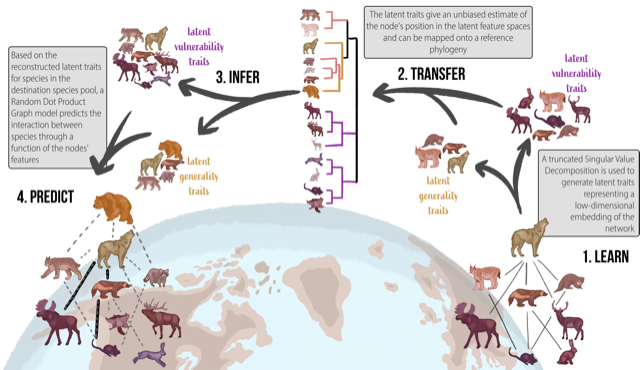
\includegraphics[width=\textwidth]{figures/figure-concept_v2.png}
    \caption{Overview of the phylogenetic transfer learning (and prediction)
of species interactions networks. Starting from an initial, known,
network, we learn its representation through a graph embedding step
(here, a truncated Singular Value Decomposition; Step 1), yielding a
series of latent traits (latent vulnerability traits are more
representative of species at the lower trophic-level and latent
generality traits are more representative of species at higher
trophic-levels; \emph{sensu} \cite{Schoener1989Food}); second, for the
destination species pool, we perform ancestral character estimation
using a phylogeny (here, using a Brownian model for the latent traits;
Step 2); we then sample from the reconstructed distribution of latent
traits (Step 3) to generate a probabilistic metaweb at the destination
(here, assuming a uniform distribution of traits), and threshold it to
yield the final list of interactions (Step 4).}
    \label{fig:concept}
\end{figure}

In \autoref{fig:concept}, we provide a methodological overview based on learning
the embedding of a metaweb of trophic interactions for European mammals
(known interactions; \cite{Maiorano2020Tetraeu, Maiorano2020Data}) and,
based on phylogenetic relationships between mammals globally \emph{i.e.,}
phylogenetic tree (\cite{Upham2019Inferring}), infer a metaweb for the Canadian
mammalian species pool (using only a species list \emph{i.e.,} we have no
prior data on species interaction data for Canada in this instance). Our
case study shows that phylogenetic transfer learning is an effective
approach to the generation of probabilistic metawebs. This showcases
that although the components (species) that make up the Canadian and
European communities may be \emph{minimally} shared (the overall species
overlap is less than 4\%), if the medium (proxy space) selected in the
transfer step is biologically plausible, we can still effectively learn
from the known network and make biologically relevant predictions of
interactions. Indeed, as we detail in the results, when validated
against the known (but fractional) data of trophic interactions present
between Canadian mammals, our model achieves a predictive accuracy of
approximately 91\%.

\section{Method description}\label{method-description}

The core point of our method is the transfer of knowledge of a known
ecological network to predict interactions between species for another
location for which the network is unknown (or partially known) and is
summarized in the grey text boxes in \autoref{fig:concept}. The method we develop
is, ecologically speaking, a ``black box'', \emph{i.e.,} an algorithm
that can be understood mathematically, but whose component parts are not
always directly tied to ecological processes. There is a growing
realization in machine learning that (unintentional) black box
algorithms are not necessarily a bad thing (\cite{Holm2019Defense}), as
long as their constituent parts can be examined (which is the case with
our method). But more importantly, data hold more information than we
might think; as such, even algorithms that are disconnected from a model
can make correct guesses most of the time (\cite{Halevy2009Unreasonable}); in
fact, in an instance of ecological forecasting of spatio-temporal
systems, model-free approaches (\emph{i.e.,} drawing all of their
information from the data) outperformed model-informed ones
(\cite{Perretti2013Modelfree}).

\subsection{Data used for the case
study}\label{data-used-for-the-case-study}

We use data from the European metaweb assembled by \cite{Maiorano2020Tetraeu}.
This was assembled using data extracted from scientific literature
(including published papers, books, and grey literature) from the last
50 years and includes all terrestrial tetrapods (mammals, breeding
birds, reptiles and amphibians) occurring on the European sub-continent
(and Turkey) - with the caveat that only species introduced in
historical times and currently naturalized being included. The European
metaweb was filtered using the Global Biodiversity Information Facility
(GBIF) taxonomic backbone (\cite{GBIFSecretariat2021Gbif}) so as to
contain only terrestrial and semi-aquatic mammals. As all species had
valid matches to the GBIF taxonomy it was used as the backbone for the
remaining reconciliation steps namely, the mammalian consensus supertree
by \cite{Upham2019Inferring} (which is used for the knowledge transfer step) and for the Canadian species list---which was extracted from the
International Union for Conservation of Nature (IUCN) checklist, and
corresponds to the same selection criteria that was applied by
\cite{Maiorano2020Tetraeu} in the European metaweb. After taxonomic cleaning
and reconciliation the European metaweb has 260 species, and the
Canadian species pool 163; of these, 17 (about 4\% of the total) are
shared, and 89 species from Canada (54\%) had at least one congeneric
species in Europe. The similarity for both species pools predictably
increases with higher taxonomic order, with 19\% of shared genera, 47\%
of shared families, and 75\% of shared orders; for the last point,
Canada and Europe each had a single unique order (\emph{Didelphimorphia}
for Canada, \emph{Erinaceomorpha} for Europe).

\subsection{Implementation and code
availability}\label{implementation-and-code-availability}

The entire pipeline is implemented in \texttt{Julia} 1.6
(\cite{Bezanson2017Julia}) and is available under the permissive MIT
License at \href{https://osf.io/2zwqm/}{\texttt{https://osf.io/2zwqm/}}.
The taxonomic cleanup steps are done using \texttt{GBIF.jl}
(\cite{Dansereau2021Simplesdmlayers}). The network embedding and analysis is done
using \texttt{EcologicalNetworks.jl} (\cite{Banville2021Mangal,,
Poisot2019EcoJl}). The phylogenetic simulations are done using
\texttt{PhyloNetworks.jl} (\cite{Solis-Lemus2017Phylonetworks}) and
\texttt{Phylo.jl} (\cite{Reeve2016How}). A complete
\texttt{Project.toml} file specifying the full tree of dependencies is
available alongside the code. This material also includes a fully
annotated copy of the entire code required to run this project
(describing both the intent of the code and discussing some technical
implementation details), a vignette for every step of the process, and a
series of Jupyter notebooks with the text and code. The pipeline can be
executed on a laptop in a matter of minutes, and therefore does not
require extensive computational power.

\subsection{Step 1: Learning the origin network
representation}\label{step-1-learning-the-origin-network-representation}

The first step in transfer learning is to learn the structure of the
original dataset. In order to do so, we rely on an approach inspired
from representational learning, where we learn a \emph{representation}
of the metaweb (in the form of the latent subspaces), rather than a list
of interactions (species \emph{a} eats \emph{b}). This approach is
conceptually different from other metaweb-scale predictions (\emph{e.g.,}
\cite{Albouy2019Marine}), in that the metaweb representation is easily
transferable. Specifically, we use a Random Dot Product Graph model
(hereafter RDPG; \cite{Young2007Random}) to create a number of latent
variables that can be combined into an approximation of the network
adjacency matrix. RDPG is known to capture the evolutionary backbone of
food webs (\cite{DallaRiva2016Exploring}), resulting in strong phylogenetic
signal in RDPG results; in other words, the latent variables of an RDPG
can be mapped onto a phylogenetic tree, and phylogenetically similar
predators should share phylogenetically similar preys. In addition,
recent advances show that the latent variables produced this way can be
used to predict \emph{de novo} interactions. Interestingly, the latent
variables do not need to be produced by decomposing the network itself;
in a recent contribution, (\cite{Runghen2021Exploiting}) showed that deep artificial
neural networks are able to reconstruct the left and right subspaces of
an RDPG, in order to predict human movement networks from
individual/location metadata and opens up the possibility of using
additional metadata as predictors.

The latent variables are created by performing a truncated Singular
Value Decomposition (t-SVD; \cite{Halko2011Finding}) on the adjacency
matrix. SVD is an appropriate embedding of ecological networks, which
has recently been shown to both capture their complex, emerging
properties (\cite{Strydom2021SvdEnt}) and to allow highly accurate
prediction of the interactions within a single network
(\cite{Poisot2021ImpMam}). Under SVD, an adjacency matrix \(\mathbf{A}\)
(where \(\mathbf{A}_{m,n}\in\mathbb{B}\) where 1 indicates predation and
0 an absence thereof) is decomposed into three components resulting in
\(\mathbf{A} = \mathbf{U}\mathbf{\Sigma}\mathbf{V'}.\) Here,
\(\mathbf{\Sigma}\) is a \(m \times n\) diagonal matrix and contains
only singular (\(\sigma\)) values along its diagonal, \(\mathbf{U}\) is
a \(m \times m\) unitary matrix, and \(\mathbf{V}'\) a \(n \times n\)
unitary matrix. Truncating the SVD removes additional noise in the
dataset by omitting non-zero and/or smaller \(\sigma\) values from
\(\mathbf{\Sigma}\) using the rank of the matrix. Under a t-SVD
\(\mathbf{A}_{m,n}\) is decomposed so that \(\mathbf{\Sigma}\) is a
square \(r \times r\) diagonal matrix (with \(1 \le r \le r_{full}\)
where \(r_{full}\) is the full rank of \(\mathbf{A}\) and \(r\) the rank
at which we truncate the matrix) containing only non-zero \(\sigma\)
values. Additionally, \(\mathbf{U}\) is now an \(m \times r\) semi
unitary matrix and \(\mathbf{V}'\) an \(r \times n\) semi-unitary
matrix.

The specific rank at which the SVD ought to be truncated is a difficult
question. The purpose of SVD is to remove the noise (expressed at high
dimensions) and to focus on the signal (expressed at low dimensions). In
datasets with a clear signal/noise demarcation, a scree plot of
\(\mathbf{\Sigma}\) can show a sharp drop at the rank where noise starts
(\cite{Zhu2006Automatic}). Because the European metaweb is almost entirely
known, the amount of noise (uncertainty) is low; this is reflected in
Fig.\ref{fig:scree} (left), where the scree plot shows no important drop, and in
Fig.\ref{fig:scree} (right) where the proportion of variance explained increases
smoothly at higher dimensions. For this reason, we default back to a
threshold that explains 60\% of the variance in the underlying data,
corresponding to 12 dimensions - \emph{i.e.,} a tradeoff between accuracy
and a reduced number of features.

An RDPG estimates the probability of observing interactions between
nodes (species) as a function of the nodes' latent variables, and is a
way to turn an SVD (which decompose one matrix into three) into two
matrices that can be multiplied to provide an approximation of the
network. The latent variables used for the RDPG, called the left and
right subspaces, are defined as
$\mathscr{L} = \mathbf{U}\sqrt{\mathbf{\Sigma}}$, and
$\mathscr{R} = \sqrt{\mathbf{\Sigma}}\mathbf{V}'$ -- using the full
rank of $\mathbf{A}, \mathscr{L}\mathscr{R} = \mathbf{A}$, and
using any smaller rank results in
$\mathscr{L}\mathscr{R} \approx \mathbf{A}$. Using a rank of 1 for the
t-SVD provides a first-order approximation of the network. One advantage
of using an RDPG for the network reconstruction rather than an SVD is
that the number of components to estimate decreases; notably, one does
not have to estimate the singular values of the SVD. Furthermore, the
two subspaces can be directly multiplied to yield a network.

\begin{figure}[h]
    \centering
    \includegraphics[width=\textwidth]{figures/figure-screeplot.png}
    \caption{Left: representation of the scree plot of the singular values
from the t-SVD on the European metaweb. The scree plot shows no obvious
drop in the singular values that may be leveraged to automatically
detect a minimal dimension for embedding, after \emph{e.g.,}
\cite{Zhu2006Automatic}. Right: cumulative fraction of variance explained by each
dimension up to the rank of the European metaweb. The grey lines
represent cutoffs at 50, 60, \ldots, 90\% of variance explained. For the
rest of the analysis, we reverted to an arbitrary threshold of 60\% of
variance explained, which represented a good tradeoff between accuracy
and reduced number of features.}
    \label{fig:scree}
\end{figure}

Because RDPG relies on matrix multiplication, the higher dimensions
essentially serve to make specific interactions converge towards 0 or 1;
therefore, for reasonably low ranks, there is no guarantee that the
values in the reconstructed network will be within the unit range. In
order to determine what constitutes an appropriate threshold for
probability, we performed the RDPG approach on the European metaweb, and
evaluated the probability threshold by treating this as a binary
classification problem, specifically assuming that both 0 and 1 in the
European metaweb are all true. Given the methodological details given in
\cite{Maiorano2020Tetraeu} and \cite{OConnor2020Unveiling}, this seems like a reasonable
assumption, although one that does not hold for all metawebs. We used
the thresholding approach presented in \cite{Poisot2021ImpMam}, and picked a
cutoff that maximized Youden's \(J\) statistic (a measure of the
informedness (trust) of predictions; \cite{Youden1950Index}); the resulting
cutoff was 0.22, and gave an accuracy above 0.99. In \autoref{svd-does-not-overfit-on-the-european-network}, we
provide several lines of evidence that using the entire network to
estimate the threshold does not lead to overfitting; that using a subset
of species would yield the same threshold; that decreasing the quality
of the original data by adding or removing interactions would minimally
affect the predictive accuracy of RDPG applied to the European metaweb;
and that the networks reconstructed from artificially modified data are
reconstructed with the correct ecological properties.

The left and right subspaces for the European metaweb, accompanied by
the threshold for prediction, represent the knowledge we seek to
transfer. In the next section, we explain how we rely on phylogenetic
similarity to do so.

\subsection{Steps 2 and 3: Transfer learning through phylogenetic
relatedness}\label{steps-2-and-3-transfer-learning-through-phylogenetic-relatedness}

In order to transfer the knowledge from the European metaweb to the
Canadian species pool, we performed ancestral character estimation using
a Brownian motion model, which is a conservative approach in the absence
of strong hypotheses about the nature of phylogenetic signal in the
network decomposition (\cite{Litsios2012Effects}). This uses the estimated
feature vectors for the European mammals to create a state
reconstruction for all species (conceptually something akin to a
trait-based mammalian phylogeny using latent generality and
vulnerability traits) and allows us to impute the missing (latent) trait
data for the Canadian species that are not already in the European
network; as we are focused on predicting contemporary interactions, we
only retained the values for the tips of the tree. We assumed that all
traits (\emph{i.e.,} the feature vectors for the left and right
subspaces) were independent, which is a reasonable assumption as every
trait/dimension added to the t-SVD has an \emph{additive} effect to the
one before it. Note that the \cite{Upham2019Inferring} tree itself has some
uncertainty associated to inner nodes of the phylogeny. In this case
study we have decided to not propagate this uncertainty as it would
complexify the process. The Brownian motion algorithm returns the
\emph{average} value of the trait, and its upper and lower bounds.
Because we do not estimate other parameters of the traits'
distributions, we considered that every species trait is represented as
a uniform distribution between these bounds. The choice of the uniform
distribution was made because the algorithm returns a minimum and
maximum point estimate for the value, and given this information, the
uniform distribution is the one with maximum entropy. Had all mean
parameters estimates been positive, the exponential distribution would
have been an alternative, but this is not the case for the subspaces of
an RDPG. In order to examine the consequences of the choice of
distribution, we estimated the variance per latent variable per node to
use a Normal distribution; as we show in \autoref{the-normal-model-of-latent-variable-evolution-over-predicts}, this decision
results in dramatically over-estimating the number and probability of
interactions, and therefore we keep the discussions in the main text to
the uniform case. The inferred left and right subspaces for the Canadian
species pool ($\hat{\mathscr{L}}$) and ($\hat{\mathscr{R}}$) have
entries that are distributions, representing the range of values for a
given species at a given dimension. These objects represent the
transferred knowledge, which we can use for prediction of the Canadian
metaweb.

\subsection{Step 4: Probabilistic prediction of the destination
network}\label{step-4-probabilistic-prediction-of-the-destination-network}

The phylogenetic reconstruction of \(\hat{\mathscr{L}}\) and
\(\hat{\mathscr{R}}\) has an associated uncertainty, represented by the
breadth of the uniform distribution associated to each of their entries.
Therefore, we can use this information to assemble a
\emph{probabilistic} metaweb in the sense of \cite{Poisot2016Structure},
\emph{i.e.,} in which every interaction is represented as a single,
independent, Bernoulli event of probability \(p\).

\begin{figure}[h]
    \centering
    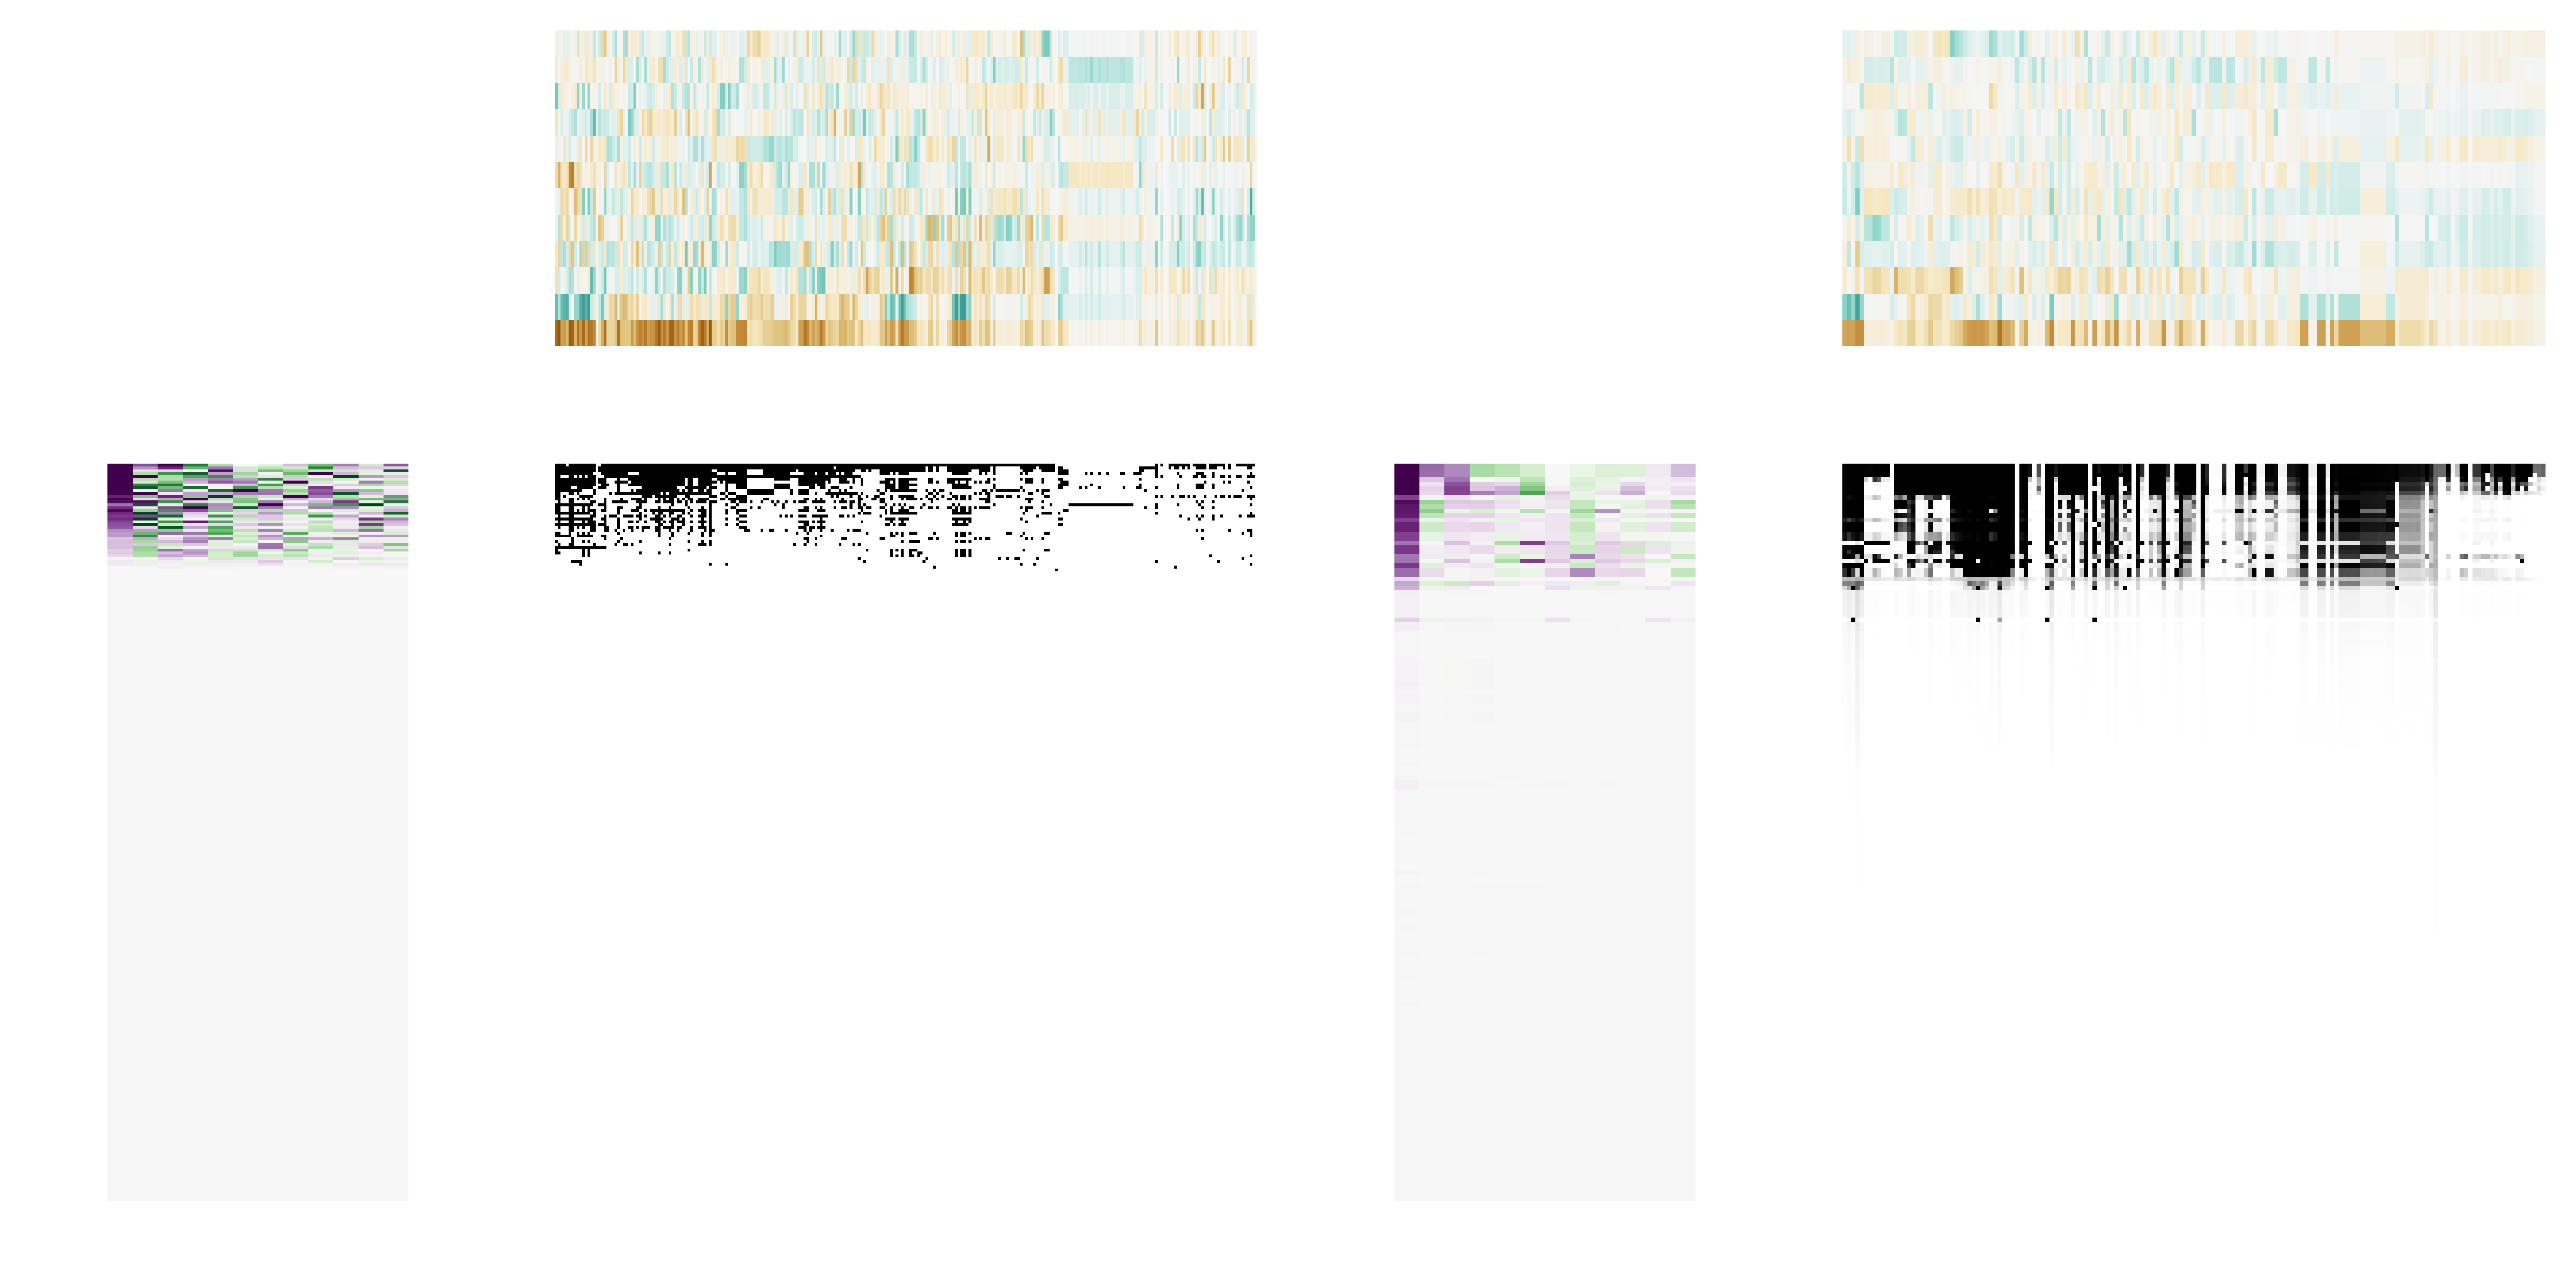
\includegraphics[width=\textwidth]{figures/figure-subspaces.png}
    \caption{Visual representation of the left (green/purple; left-side
matrix) and right (green/brown; top matrix) subspaces, alongside the
adjacency matrix of the food web they encode (grey scale). Where the
color saturation is the magnitude of the latent trait value. The
European metaweb is on the left, and the imputed Canadian metaweb
(before data inflation) on the right. This figure illustrates how much
structure the left subspace captures. As we show in \autoref{fig:degree}, the
species with a value of 0 in the left subspace are species without any
prey.}
    \label{fig:subspaces}
\end{figure}

Specifically, we have adopted the following approach. For every entry in
($\hat{\mathscr{L}}$) and ($\hat{\mathscr{R}}$), we draw a value from
its distribution. This results in one instance of the possible left
($\hat{l}$) and right ($\hat{r}$) subspaces for
the Canadian metaweb. These can be multiplied, to produce one matrix of
real values. Because the entries in $\hat{l}$ and
$\hat{r}$ are in the same space where ($\mathscr{L}$) and
($\mathscr{R}$) were originally predicted, it follows that the threshold
($\rho$) estimated for the European metaweb also applies. We use this
information to produce one random Canadian metaweb,
\(N = \hat{\mathscr{L}}\hat{\mathscr{R}}' \ge \rho\). As we can see in
(\autoref{fig:subspaces}), the European and Canadian metawebs are structurally
similar (as would be expected given the biogeographic similarities) and
the two (left and right) subspaces are distinct \emph{i.e.,} capturing
predation (generality) and prey (vulnerability) latent traits.

Because the intervals around some trait values can be broad (in fact,
probably broader than what they would actually be, see \emph{e.g.,}
\cite{Garland1999Introduction}), we repeat the above process \(2\times 10^5\)
times, which results in a probabilistic metaweb \(P\), where the
probability of an interaction (here conveying our degree of trust that
it exists given the inferred trait distributions) is given by the number
of times where it appears across all random draws \(N\), divided by the
number of samples. An interaction with \(P_{i,j} = 1\) means that these
two species were predicted to interact in all \(2\times 10^5\) random
draws.

It must be noted that despite bringing in a large amount of information
from the European species pool and interactions, the Canadian metaweb
has distinct structural properties. Following an approach similar to
\cite{Vermaat2009Major}, we show in \autoref{rdpg-reconstructed-networks-have-diverse-structures} that not only can we observe
differences in the multivariate space between the European and Canadian
metawebs, we can also observe differences in the same space between
random subgraphs from these networks. These results line up with the
studies spatializing metawebs that have been discussed in the
introduction: changes in the species pool are driving local structural
changes in the networks.

\subsection{Data cleanup, discovery, validation, and
thresholding}\label{data-cleanup-discovery-validation-and-thresholding}

Once the probabilistic metaweb for Canada has been produced, we followed
a number of data inflation steps to finalize it. This step is external
to the actual transfer learning framework but rather serves as a way to
augment and validate the predicted metaweb.

\begin{figure}[h]
    \centering
    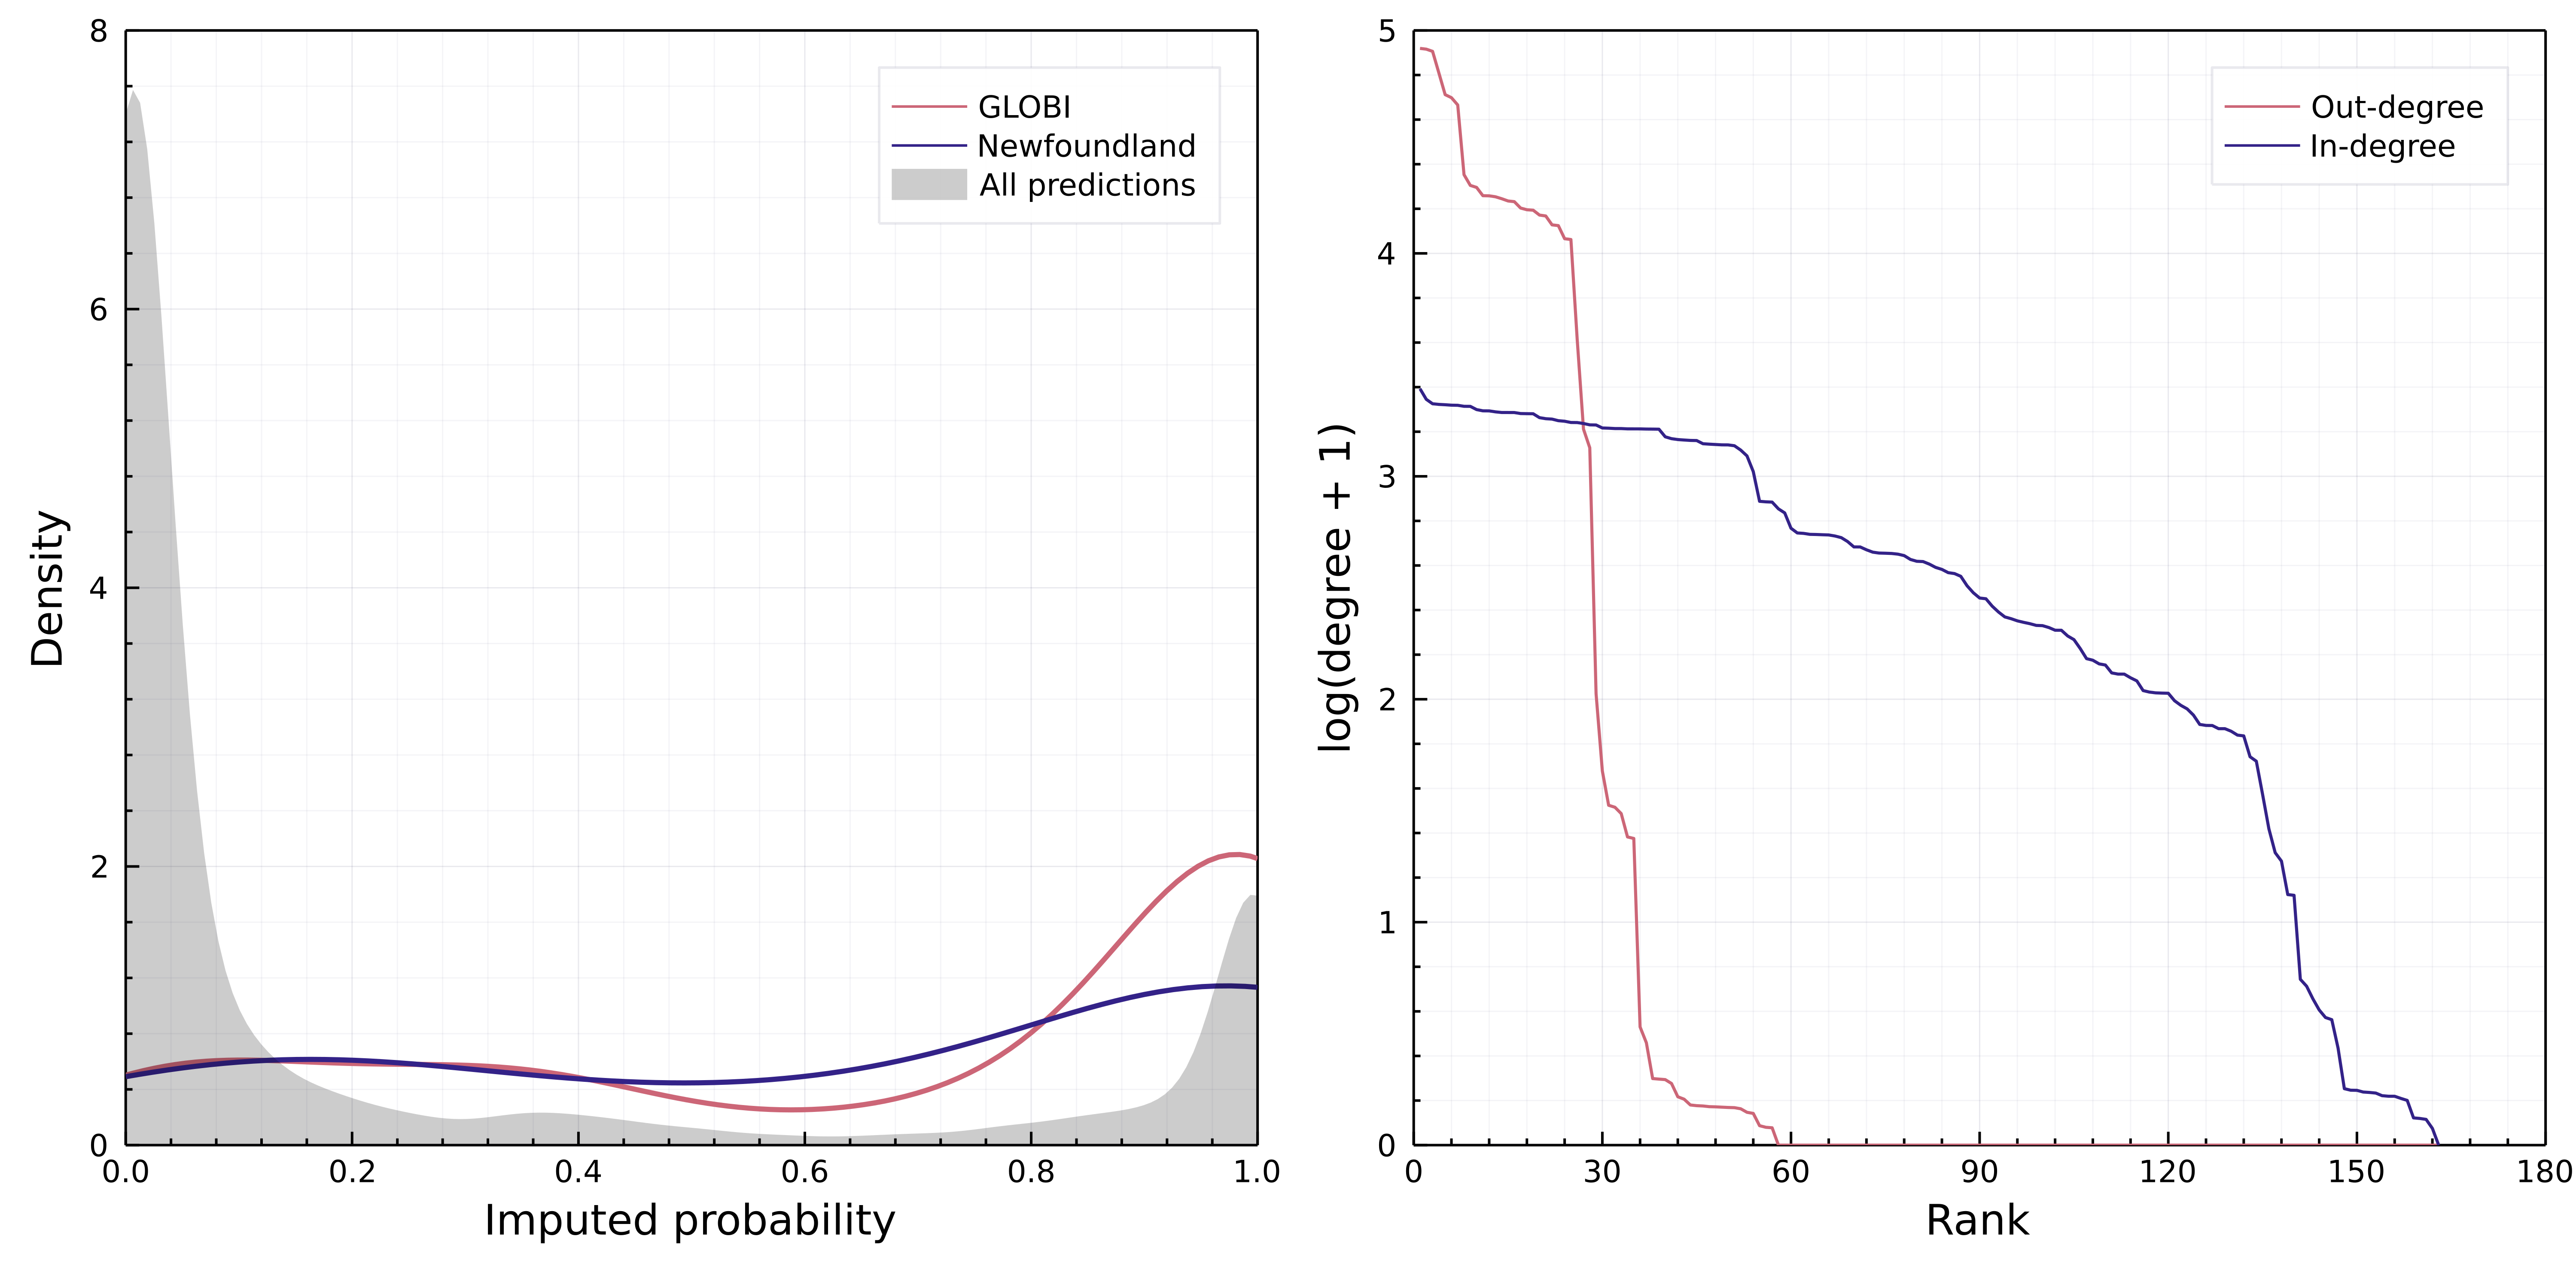
\includegraphics[width=\textwidth]{figures/figure-validation.png}
    \caption{Left: comparison of the probabilities of interactions assigned
by the model to all interactions (grey curve), the subset of
interactions found in GloBI (red), and in the \cite{Strong2014Impact}
Newfoundland dataset (blue). The model recovers more interactions with a
low probability compared to data mining, which can suggest that
collected datasets are biased towards more common or easy to identify
interactions. Right: distribution of the in-degree and out-degree of the
mammals from Canada in the reconstructed metaweb, where the rank is the
maximal number of linearly independent columns (interactions) in the
metaweb. This figure describes a flat, relatively short food web, in
which there are few predators but a large number of
preys.}
    \label{fig:inflation}
\end{figure}

First, we extracted the network corresponding to the 17 species shared
between the European and Canadian pools and replaced these interactions
with a probability of 0 (non-interaction) or 1 (interaction), according
to their value in the European metaweb. This represents a minute
modification of the inferred network (about 0.8\% of all species pairs
from the Canadian web), but ensures that we are directly re-using
knowledge from Europe.

Second, we looked for all species in the Canadian pool known to the
Global Biotic Interactions (GloBI) database \cite{Poelen2014Global}), and
extracted their known interactions. Because GloBI aggregates observed
interactions, it is not a \emph{networks} data source, and therefore the
only information we can reliably extract from it is that a species pair
\emph{was reported to interact at least once}. This last statement
should yet be taken with caution, as some sources in GloBI (\emph{e.g.,}
\cite{Thessen2014Knowledge}) are produced through text analysis, and therefore
may not document direct evidence of the interaction. Nevertheless,
should the predictive model work, we would expect that a majority of
interactions known to GloBI would also be predicted. We retrieved 366
interactions between mammals from the Canadian species pool from GloBI,
33 of which were not predicted by the model; this results in a success
rate of 91\%. After performing this check, we set the probability of all
interactions known to GloBI to 1.

Finally, we downloaded the data from \cite{Strong2014Impact}, who mined
various literature sources to identify trophic interactions in
Newfoundland. This dataset documented 25 interactions between mammals,
only two of which were not part of our (Canada-level) predictions,
resulting in a success rate of 92\%. These two interactions were added
to our predicted metaweb with a probability of 1. A comparison of
interaction densities for the inferred metaweb, and the Globi and
Newfoundland is shown in Fig.\ref{fig:inflation} and a table listing all
interactions in the predicted Canadian metaweb can be found in the
supplementary material.

\begin{figure}[h]
    \centering
    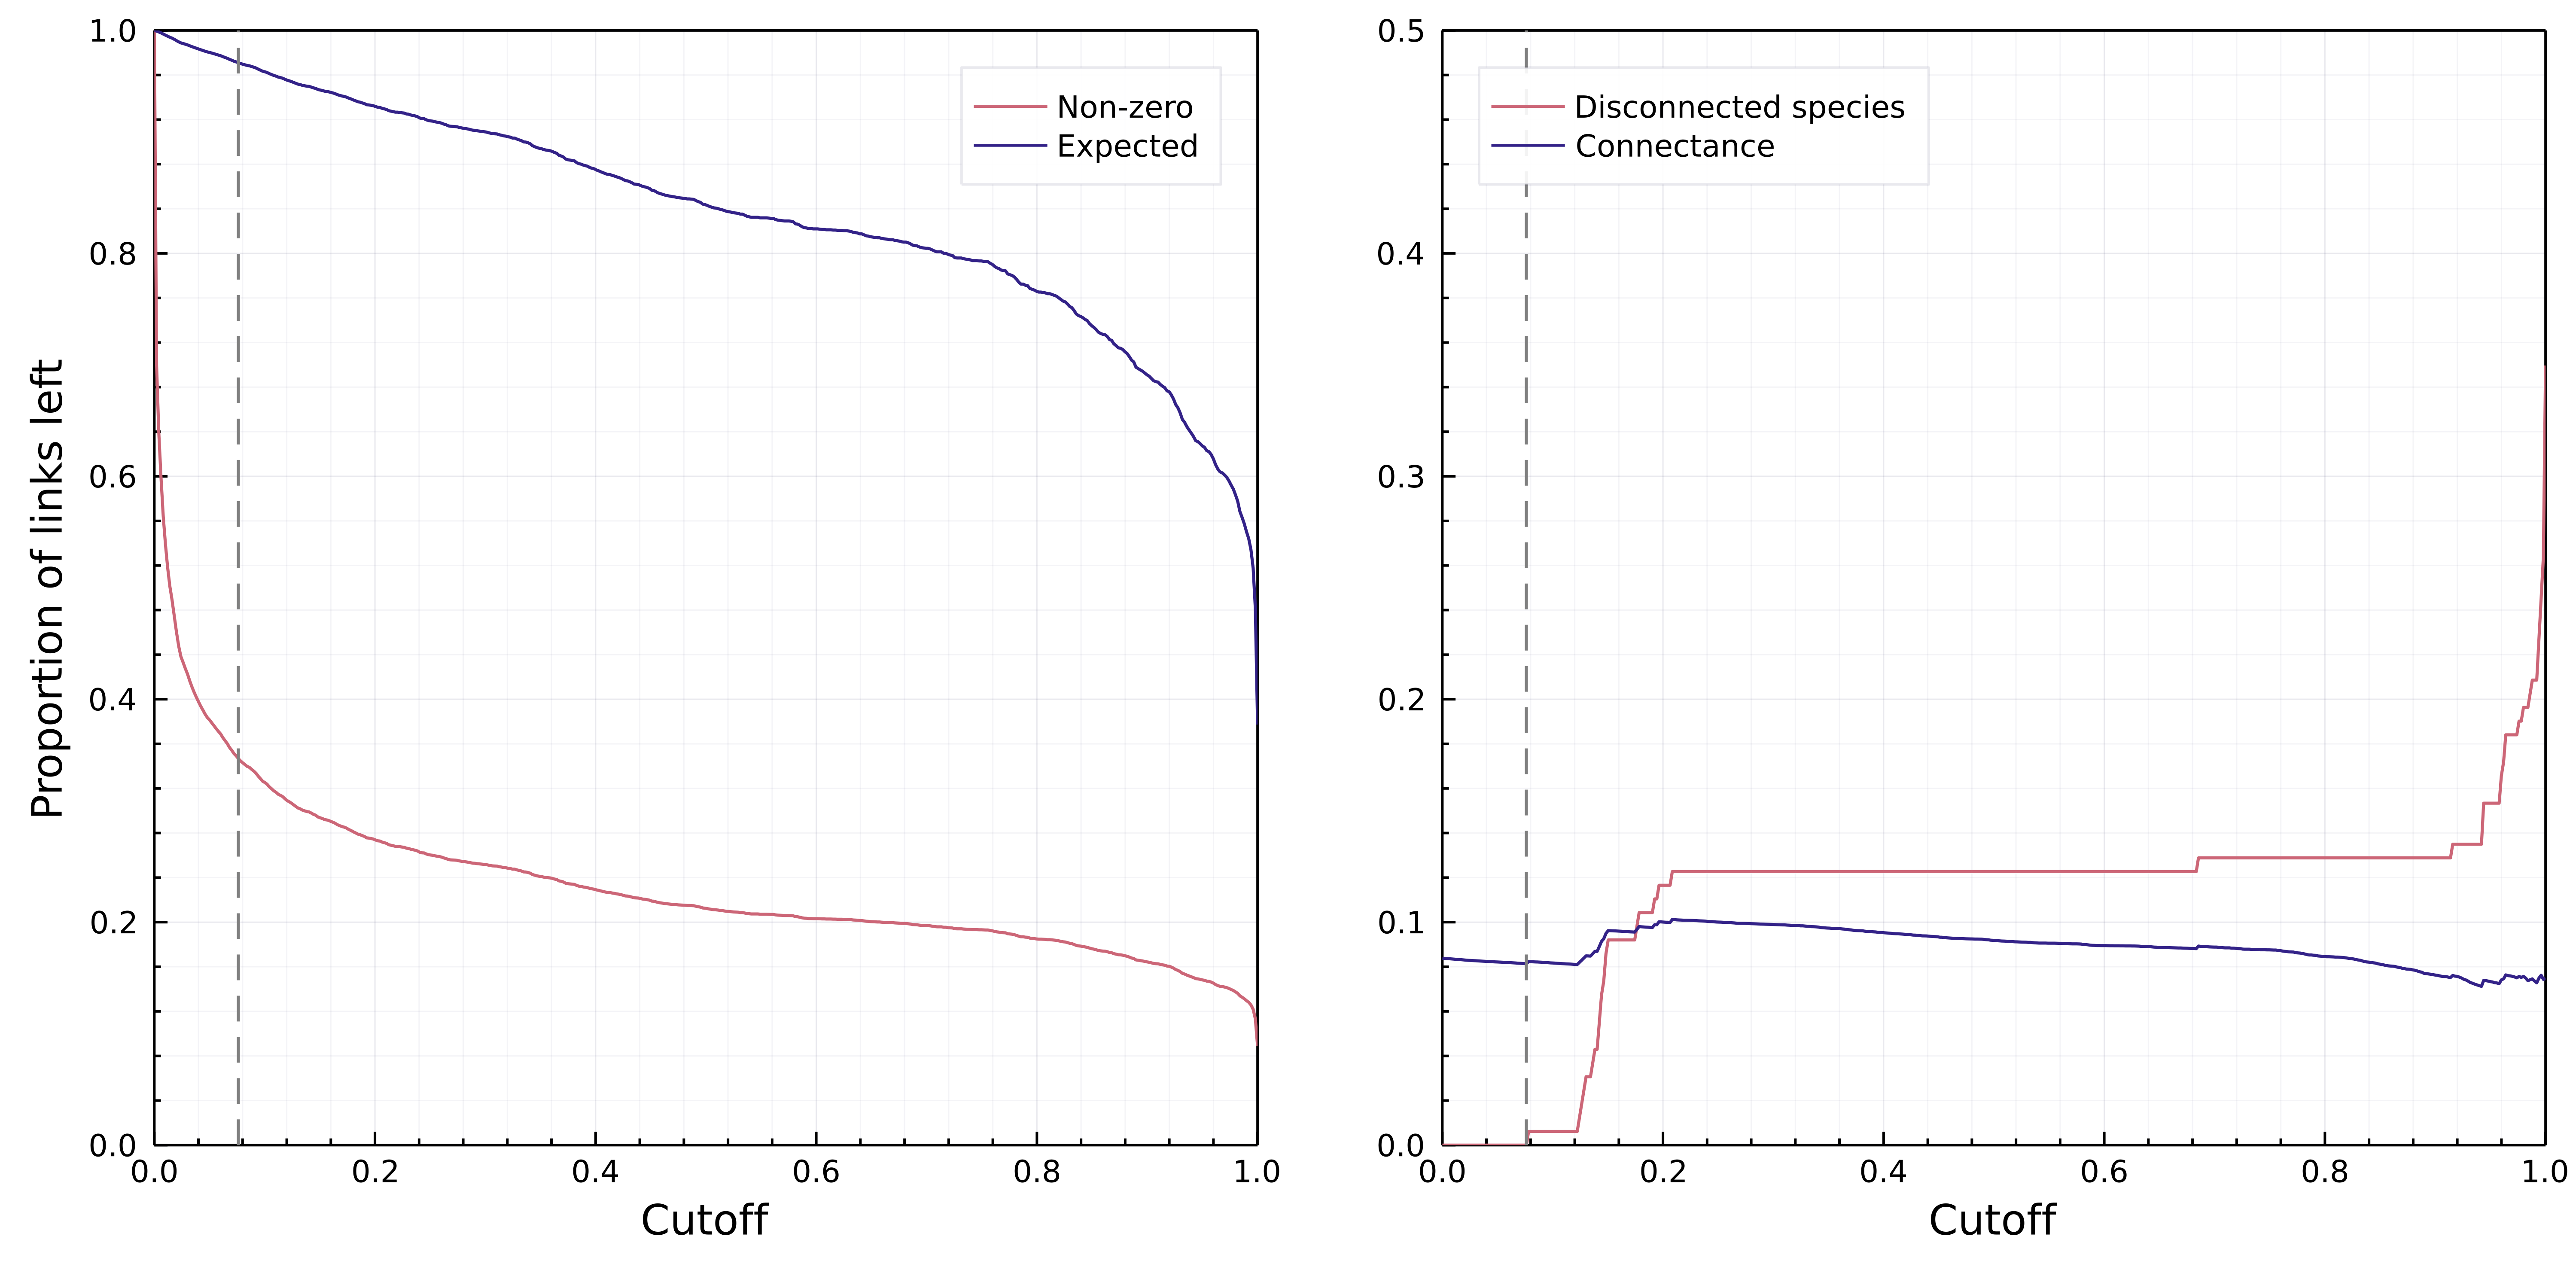
\includegraphics[width=\textwidth]{figures/figure-cutoffs.png}
    \caption{Left: effect of varying the cutoff for probabilities to be
considered non-zero on the number of unique links and on \(\hat{L}\),
the probabilistic estimate of the number of links assuming that all
interactions are independent. Right: effect of varying the cutoff on the
number of disconnected species, and on network connectance. In both
panels, the grey line indicates the cutoff
\(P(i\rightarrow j) \approx 0.08\) that resulted in the first species
losing all of its interactions.}
    \label{fig:thresholds}
\end{figure}

Because the confidence intervals on the inferred trait space are
probably over-estimates, we decided to apply a thresholding step to the
interactions after data inflation (see Fig.\ref{fig:thresholds} showing the
effect of varying the cutoff on \(P(i \rightarrow j)\)).
\cite{Cirtwill2021Building} proposed a number of strategies to threshold
probabilistic networks. Their methodology assumes the underlying data to
be tag-based sequencing, which represents interactions as co-occurrences
of predator and prey within the same tags; this is conceptually
identical to our Bernoulli-trial based reconstruction of a probabilistic
network. We performed a full analysis of the effect of various cutoffs,
and as they either resulted in removing too few interactions, or
removing enough interactions that species started to be disconnected
from the network, we set this threshold for a probability equivalent to
0 to the largest possible value that still allowed all species to have
at least one interaction with a non-zero probability. The need for this
slight deviation from the \cite{Cirtwill2021Building} methodology highlights the need for additional development on network thresholding.

\section{Results and discussion}\label{results-and-discussion}

\begin{figure}[h]
    \centering
    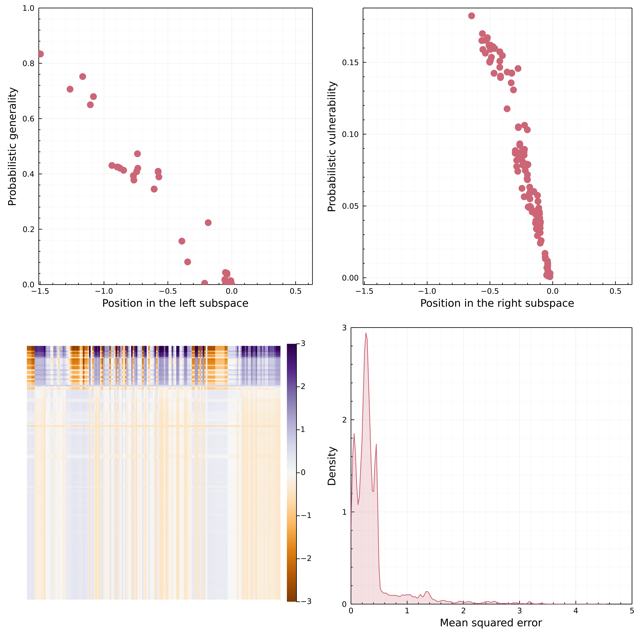
\includegraphics[width=\textwidth]{figures/figure-degree.png}
    \caption{Top: biological significance of the first dimension. Left:
there is a linear relationship between the values on the first dimension
of the left subspace and the generality, \emph{i.e.,} the relative number
of preys, \emph{sensu} \cite{Schoener1989Food}. Species with a value of 0 in
this subspace are at the bottom-most trophic level. Right: there is,
similarly, a linear relationship between the position of a species on
the first dimension of the right subspace and its vulnerability,
\emph{i.e.,} the relative number of predators. Taken together, these two
figures show that the first-order representation of this network would
capture its degree distribution. Bottom: topological consequences of the
first dimension. Left: differences in the \(z\)-scores of the actual
configuration model for the reconstructed network and the prediction
based only on the first dimension (with a deeper saturation indicating a
bigger difference in scores). Right: distribution of the differences in
the left panel.}
    \label{fig:degree}
\end{figure}

Using a transfer learning framework we were able to construct a
probabilistic metaweb and (as per \cite{Dunne2006Network}) is a list of
potential interactions, meaning that they will not necessarily be
realized wherever the two species co-occur. The t-SVD embedding is able
to learn relevant ecological features for the network. Fig.\ref{fig:degree} shows
that the first rank correlates linearly with generality and
vulnerability (\cite{Schoener1989Food}), \emph{i.e.,} the number of preys
and predators for each species. Importantly, this implies that a rank 1
approximation represents the configuration model for the metaweb,
\emph{i.e.,} a set of random networks generated from a given degree
sequence (\cite{Park2004Statistical}). Accounting for the probabilistic nature
of the degrees, the rank 1 approximation also represents the \emph{soft}
configuration model (\cite{vanderHoorn2018Sparse}). Both models are
maximum entropy graph models (\cite{Garlaschelli2018Covariance}), with sharp
(all network realizations satisfy the specified degree sequence) and
soft (network realizations satisfy the degree sequence on average) local
constraints, respectively. The (soft) configuration model is an unbiased
random graph model widely used by ecologists in the context of null
hypothesis significance testing of network structure (\emph{e.g.,}
\cite{Bascompte2003Nested}) and can provide informative priors for Bayesian
inference of network structure (\emph{e.g.,} \cite{Young2021Bayesian}). It is
noteworthy that for this metaweb, the relevant information was extracted
at the first rank. Because the first rank corresponds to the leading
singular value of the system, the results of Fig.\ref{fig:degree} have a
straightforward interpretation: degree-based processes are the most
important in structuring the mammalian food web.

One important aspect in which Europe and Canada differ (despite their
comparable bioclimatic conditions) is the degree of the legacy of human
impacts, which have been much longer in Europe. \cite{Nenzen2014Impact} showed
that even at small scales (the Iberian peninsula), mammal food webs
retain the signal of both past climate change and human activity, even
when this human activity was orders of magnitude less important than it
is now. Similarly, \cite{Yeakel2014Collapse} showed that changes in human
occupation over several centuries can lead to food web collapse.
Megafauna in particular seems to be very sensitive to human arrival
(\cite{Pires2015Pleistocene}). In short, there is well-substantiated support
for the idea that human footprint affects more than the risk of species
extinction (\cite{Marco2018Changes}), and can lead to changes in
interaction structure.

\cite{Cirtwill2019QuaFra} showed that network inference techniques based on
Bayesian approaches would perform far better in the presence of an
interaction-level informative prior; the desirable properties of such a
prior would be that it is expressed as a probability, preferably
representing a Bernoulli event, the value of which would be
representative of relevant biological processes (probability of
predation in this case). We argue that the probability returned at the
very last step of our framework may serve as this informative prior;
indeed, the output of our analysis can be used in subsequent steps, also
possibly involving expert elicitation to validate some of the most
strongly recommended interactions. One important \emph{caveat} to keep
in mind when working with interaction inference is that interactions can
never really be true negatives (in the current state of our
methodological framework and data collection limitations); this renders
the task of validating a model through the usual application of binary
classification statistics very difficult (although see
\cite{Strydom2021Roadmap} for a discussion of alternative suggestions). The
other way through which our framework can be improved is by substituting
the predictors that are used for transfer. For example, in the presence
of information on species traits that are known to be predictive of
species interactions, one might want to rely on functional rather than
phylogenetic distances -- in food webs, body size (and allometrically
related variables) has been established as such a variable
(\cite{Brose2006Consumer}); the identification of relevant functional traits
is facilitated by recent methodological developments
(\cite{Rosado2013Going}).

Finally, it should be noted that the framework we have presented is
amenable to changes lending to applicability to a broad range of
potential scenarios. For example in this case study we have embedded the
original metaweb using t-SVD, because it lends itself to an RDPG
reconstruction, which is known to capture the consequences of
evolutionary processes (\cite{DallaRiva2016Exploring}); this being said,
there are other ways to embed graphs (\cite{Arsov2019Network, Cai2017Comprehensive, Cao2019Network}), which can be used as alternatives.
Regarding the transfer step it is possible to use distinct trees if
working with distinct clades (such as pollination networks) or an
alternative measure of similarity (transfer medium) such as information
on foraging (\cite{Beckerman2006Foraging}), cell-level mechanisms
(\cite{Boeckaerts2021Predicting}), or a combination of traits and phylogenetic
structure (\cite{Stock2021Pairwise}). Most importantly, although we focus on
a trophic system, it is an established fact that different (non-trophic)
interactions do themselves interact with and influence the outcome of
trophic interactions (see \emph{e.g.,} \cite{Kawatsu2021Are, Kefi2012More}). Future development of metaweb inference techniques
should cover the prediction of multiple interaction types.

\textbf{Acknowledgements:} We acknowledge that this study was conducted
on land within the traditional unceded territory of the Saint Lawrence
Iroquoian, Anishinabewaki, Mohawk, Huron-Wendat, and Omàmiwininiwak
nations. TP, TS, DC, and LP received funding from the Canadian Institute
for Ecology \& Evolution. FB is funded by the Institute for Data
Valorization (IVADO). TS, SB, and TP are funded by a donation from the
Courtois Foundation. CB was awarded a Mitacs Elevate Fellowship no.
IT12391, in partnership with fRI Research, and also acknowledges funding
from Alberta Innovates and the Forest Resources Improvement Association
of Alberta. M-JF acknowledges funding from NSERC Discovery Grant and
NSERC CRC. RR is funded by New Zealand's Biological Heritage Ngā Koiora
Tuku Iho National Science Challenge, administered by New Zealand
Ministry of Business, Innovation, and Employment. BM is funded by the
NSERC Alexander Graham Bell Canada Graduate Scholarship and the FRQNT
master's scholarship. LP acknowledges funding from NSERC Discovery Grant
(NSERC RGPIN-2019-05771). TP acknowledges financial support from NSERC
through the Discovery Grants and Discovery Accelerator Supplement
programs. MJF is supported by an NSERC PDF and an RBC Post-Doctoral
Fellowship

\printbibliography
\end{refsection}

\endinput
%%
%% End of file `article1.tex'.
